\begin{frame}
	\vspace{2cm}
	\begin{center}
		{\Huge\textbf{\textcolor{copenhagenred}{Rejection Sampling}}}
		\vspace{1cm}

		\rule{4cm}{3pt}
		\vspace{2cm}
	\end{center}
\end{frame}

\begin{frame}{Introduction}

	\textbf{Context:} Transformation methods for sampling cannot be applied

	\vspace{0.5cm}
	\textbf{Goal:} Sample from target distribution with density $\pi(x)$ where no direct
	sampling is feasible.

	\vspace{0.5cm}
	\textbf{Basic idea:} Sample from instrumental proposal $q \neq \pi$; correct
	through rejection step to obtain a sample from $\pi$.

	\vspace{0.5cm}
	\textbf{Requirements:} Given two densities $\pi,q$ with $\pi ( x ) \leq M q ( x )$ 
	for all $x$, and some $M$ where we note that $M$ is larger than 1 since 
	both $\pi$ and $q$ integrate to 1.
\end{frame}

\begin{frame}{Intuition and Algorithm}
	\begin{columns}
		\column{0.45\textwidth}
		\textbf{Intuition:}
		\begin{itemize}
			\item Throw darts uniformly under $M \cdot q(x)$
			\item Keep only those under $\pi(x)$
			\item Kept points follow $\pi(x)$ exactly!
		\end{itemize}

		\vspace{0.2cm}
		\textbf{The Algorithm:}
		\begin{enumerate}
			\item Sample $X \sim q(x)$
			\item Sample $U \sim \text{Uniform}(0,1)$
			\item Accept if $U \leq \frac{\pi(X)}{M \cdot q(X)}$
		\end{enumerate}

		\vspace{0.2cm}
		\textbf{Why it works:} We're sampling uniformly from the area under $\pi(x)$!

		\column{0.45\textwidth}
		\begin{center}
			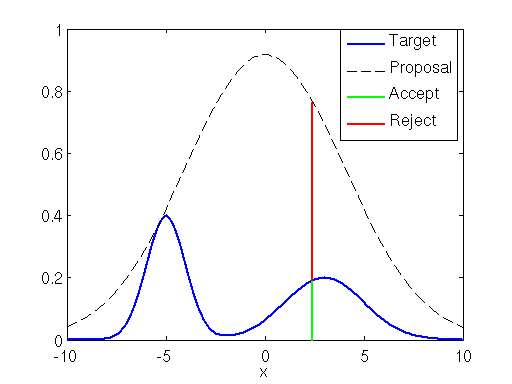
\includegraphics[width=0.95\textwidth]{rejectionsamplingcriterion.png}
		\end{center}
	\end{columns}
\end{frame}

\begin{frame}{Mathematical Foundation}
	\begin{proposition}
		The distribution of accepted samples is exactly $\pi(x)$
	\end{proposition}
	\textbf{Proof:} We need to show $P(X \in A | X \text{ accepted}) = \frac{P(X \in A, X \text{ accepted})}{P(X \text{ accepted})} = \pi(A)$. 

	\begin{align*}
		P(X \in A, X \text{ accepted}) & = \int_X \int_0^1 \mathbb{I}_A(x) \cdot \mathbb{I}\left(u \leq \frac{\pi(x)}{M q(x)}\right) q(x) \, du \, dx \\
		                               & = \int_X \mathbb{I}_A(x) \cdot \frac{\pi(x)}{M q(x)} \cdot q(x) \, dx                                        \\
		                               & = \int_X \mathbb{I}_A(x) \cdot \frac{\pi(x)}{M} \, dx = \frac{\pi(A)}{M}
	\end{align*}
	Similarly, $P(X \text{ accepted}) = \frac{1}{M}$. Therefore: $P(X \in A | X \text{ accepted}) = \frac{\pi(A)/M}{1/M} = \pi(A)$.
\end{frame}

\begin{frame}{Does this work for un-normalised distributions?}
	Often we only know $\pi$ and $q$ up to some normalising constants; i.e.
	\begin{equation*}
		\tilde{\pi} = \frac{\pi}{Z_\pi} \quad \text{and} \quad \tilde{q} = \frac{q}{Z_q}
	\end{equation*}

	where $\pi$, $q$ are known but $Z_\pi$, $Z_q$ are unknown.
	We still need to be able to sample from $q(\cdot)$.
	If we can upper bound:
	\begin{equation*}
		\frac{\tilde{\pi}(x)}{\tilde{q}(x)} \leq \widetilde{M},
	\end{equation*}
	then using $\tilde{\pi}$, $\tilde{q}$ and $\widetilde{M}$ in the algorithm is correct.
	Indeed we have
	\begin{equation*}
		\frac{\tilde{\pi}(x)} {\tilde{q}(x)} \leq \widetilde{M} \iff
		\frac{\pi(x)}{q(x)} \leq \widetilde{M} \cdot \frac{Z_q}{Z_\pi} \overset{\text{def}}{=} M
	\end{equation*}
\end{frame}

\begin{frame}
	\textbf{Waiting time:} Let $T$ denote the number of pairs $( X,U )$ that have to be
	generated until $X$ is accepted for the first time. $T$ is geometrically distributed
	with parameter $1/M$ and in particular $E ( T ) = M$.

	\vspace{0.25cm}
	This is why large $M$ is disastrous - it means you waste most of your computational effort on rejected samples!

	\vspace{0.25cm}
	\textbf{Dimensionality:} Assume $\pi$ and $q$ are Gaussian densities with same mean and
	$\sigma_q > \sigma_\pi $. Here $M = (\frac{\sigma_q}{\sigma_\pi})^d$ which grows with dimension.
	Say variance is 10\% larger and $d = 100: M = 1.1^{100} \approx 14,000$ (acceptance rate $\approx 0.007\%$)

	\vspace{0.25cm}
	\textbf{Extensions:} Squeezing techniques from exercises

	\vspace{0.25cm}{\tiny
	Each trial (drawing $X$ from $q$ and $U$ from Uniform$[0,1]$) is independent. Each trial has the same probability of success (acceptance). We stop at the first success. This is exactly the setup for a geometric distribution! 
	\textbf{Why $P(\text{accept}) = 1/M$?} From the previous proof, we showed: $P(X \text{ accepted}) = \frac{1}{M}$. So each trial succeeds (accepts) with probability $1/M$.
	\textbf{Why $T \sim \text{Geometric}(1/M)$?} Think of it like coin flips: ``Heads'' = accept (probability $1/M$), ``Tails'' = reject (probability $1 - 1/M$). $T$ is the number of flips until the first heads. This is the definition of a geometric distribution! $P(T = k) = \left(1 - \frac{1}{M}\right)^{k-1} \cdot \frac{1}{M}$. We fail $(k-1)$ times, then succeed on the $k$-th try.
	\textbf{Why $E(T) = M$?} For a geometric distribution with success probability $p = 1/M$: $E(T) = \frac{1}{p} = \frac{1}{1/M} = M$.
	}
\end{frame}
